%%
%% Author: andre
%% 21/05/18
%%

% Preamble
\documentclass[11pt]{article}
\usepackage{basic}

\title{Descrição do sistema Nação Real}
\date{\today}

% Document
\begin{document}
    \maketitle
    \tableofcontents
    \listoffigures
    \newpage

    \section{Introdução}
    \label{s-intro}

    Esse sistema destina-se à melhor articulação intra e inter células. Buscamos criar um sistema de comunicação para
    que as ações estejam melhor coordenadas.

    \section[DER]{Diagrama Entidade-Relacionamento}
    \label{DER}

    \begin{figure}
        \centering
        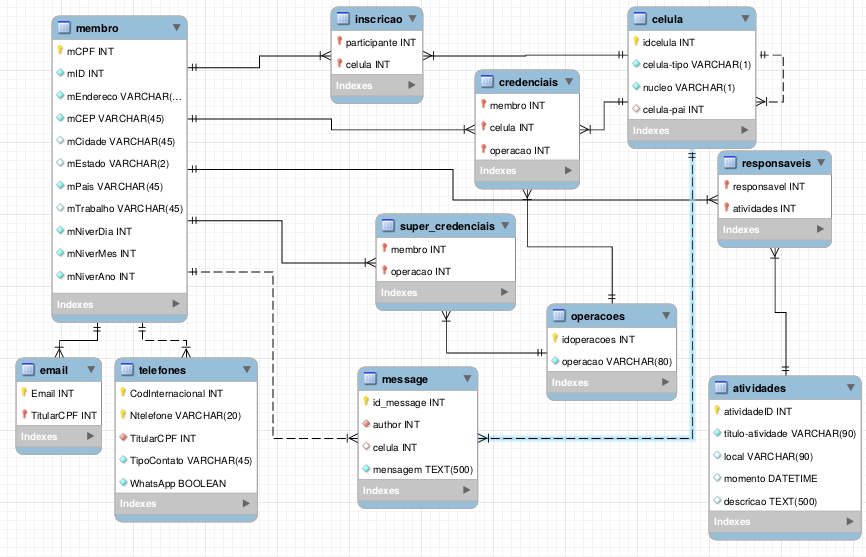
\includegraphics[width=0.85\textwidth]{bd.png}
        \caption{Diagrama que retrata as entidades}
        \label{fig:der}
    \end{figure}

    (Vide figura \ref{fig:der})

    \section[Dependências]{Descrição de dependências}

    Aqui encontra-se uma lista de dependências desse projeto:
    \begin{itemize}
        \item PostgreSQL \dir SGBD \footnote{sistema de gerenciamento de banco de dados}
        responsável pelo armazenamento de dados e transações referentes às operações de
        inserção, leitura, atualização e remoção
        \item psycopg2 \dir biblioteca Pyhton para comunicação com o SGBD
        \item Flask-RESTPlus \dir criação de rotas e requisições REST
        \item Axios \dir parte do front-end, recebem entrada em JSON e trazem os dados de
        forma nítida
        \item Vue \dir ferramenta de front-end, embelezamento
    \end{itemize}
    Abaixo encontram-se instruções de instalação. Tentarei incluir instruções de instalação
    para ambientes Unix/Linux

        \subsection{PostgreSQL}
        \subsection{Psycopg2}
        \subsection{Flask-RESTPlus}
        \subsection{Axios}
        \subsection{Vue}

    \section[Descrição]{Entidades e relacionamentos}

        \subsection{Membros}
        \subsection{Células}
        \subsection{Mensagens}
        \subsection{Atividades}
        \subsection{Operações}

    \section[Equipe]{Membros da equipe}

    Nossa equipe é formada pelos seguintes membros
    \begin{itemize}
        \item André Luiz Abdalla Silveira
        \item Insira o nome de vocês no arquivo \LaTeX
    \end{itemize}

\end{document}
